% Autor: Leonhard Segger, Alexander Neuwirth
% Datum: 2017-10-30
\documentclass[
	% Papierformat
	a4paper,
	% Schriftgröße (beliebige Größen mit „fontsize=Xpt“)
	12pt,
	% Schreibt die Papiergröße korrekt ins Ausgabedokument
	pagesize,
	% Sprache für z.B. Babel
	ngerman
]{scrartcl}

% Achtung: Die Reihenfolge der Pakete kann (leider) wichtig sein!
% Insbesondere sollten (so wie hier) babel, fontenc und inputenc (in dieser
% Reihenfolge) als Erstes und hyperref und cleveref (Reihenfolge auch hier
% beachten) als Letztes geladen werden!

\usepackage{tikz}
\usetikzlibrary{backgrounds,calc,patterns,angles,quotes} % loads some tikz extensions\usepackage{tikz}
\usetikzlibrary{babel}
% Silbentrennung etc.; Sprache wird durch Option bei \documentclass festgelegt
\usepackage{babel}
% Verwendung der Zeichentabelle T1 (Sonderzeichen etc.)
\usepackage[T1]{fontenc}
% Legt die Zeichenkodierung der Eingabedatei fest, z.B. UTF-8
\usepackage[utf8]{inputenc}
% Schriftart
\usepackage{lmodern}
% Zusätzliche Sonderzeichen
\usepackage{textcomp}

% Mathepaket (intlimits: Grenzen über/unter Integralzeichen)
\usepackage[intlimits]{amsmath}
% Ermöglicht die Nutzung von \SI{Zahl}{Einheit} u.a.
\usepackage{siunitx}
% Zum flexiblen Einbinden von Grafiken (\includegraphics)
\usepackage{graphicx}
% Abbildungen im Fließtext
\usepackage{wrapfig}
% Abbildungen nebeneinander (subfigure, subtable)
\usepackage{subcaption}
% Funktionen für Anführungszeichen
\usepackage{csquotes}
\MakeOuterQuote{"}
% Zitieren, Bibliographie
\usepackage{biblatex}


% Zur Darstellung von Webadressen
\usepackage{url}
%chemische Formeln
\usepackage[version=4]{mhchem}
% siunitx: Deutsche Ausgabe, Messfehler getrennt mit ± ausgeben
\usepackage{floatrow}
\floatsetup[table]{capposition=top}
\usepackage{float}
% Verlinkt Textstellen im PDF-Dokument
\usepackage[unicode]{hyperref}
% "Schlaue" Referenzen (nach hyperref laden!)
\usepackage{cleveref}
\sisetup{
	locale=DE,
	separate-uncertainty
}
%\bibliography{14Mo_O5_02-07-2018_References}
%TODO anpassen

\begin{document}
	
	\begin{titlepage}
		\centering
		{\scshape\LARGE Versuchsbericht zu \par}
		\vspace{1cm}
		{\scshape\huge O5 - Spektrometer \par}
		\vspace{2.5cm}
		{\LARGE Gruppe 14Mo \par}
		\vspace{0.5cm}
		
		{\large Alexander Neuwirth (E-Mail: a\_neuw01@wwu.de) \par}
		{\large Leonhard Segger (E-Mail: l\_segg03@uni-muenster.de) \par}
		\vfill
		
		durchgeführt am 04.07.2018\par
		betreut von\par
		{\large Johann Preuß} 
		
		\vfill
		
		{\large \today\par}
	\end{titlepage}
	\tableofcontents
	\newpage

	\section{Kurzfassung}
	%TODO Hypothese	und deren Ergebnis, wenn Hypothese ist, dass nur Theorie erfüllt, sagen: Erwartung: Theorie aus einführung (mit reflink) erfüllt
	%TODO Ergebnisse, auch Zahlen, mindestens wenn's halbwegs Sinn ergibt
	%TODO Was wurde gemacht
	%TODO manche leute wollen Passiv oder "man", manche nicht
	
	\section{Methoden}
	%TODO Bilder von der Website klauen
	%TODO einer will Präsens
	
	\section{Ergebnisse und Diskussion}
	%TODO Unsicherheiten
	

	\subsection{Beobachtung und Datenanalyse}
	%TODO Einflüsse von veränderten Parametern auf Messung
	\subsubsection{Unsicherheiten} %TODO GGF IN DATENANYLSY
	Die Unsicherheiten werden gemäß GUM ermittelt. 
	Außerdem wird für Unsicherheitsrechnungen die Python-Bibliothek "uncertainties" verwendet.
	\begin{description}
		\item[Winkelmessung:] 
	\end{description}
	\subsubsection{Natriumdampflampe}
	\subsubsection*{Prisma}
	Die hinter dem Prisma erkennbaren Spektrallinien sind in \cref{fig_draw} skizziert. 
	Die Spektrallinien wurden von links nach rechts stärker gebrochen.
	Auftretende Restlichteffekte ließen sich durch Abschirmung mit beispielweise den Händen entfernen. 
	\begin{figure}[H]
		\centering
		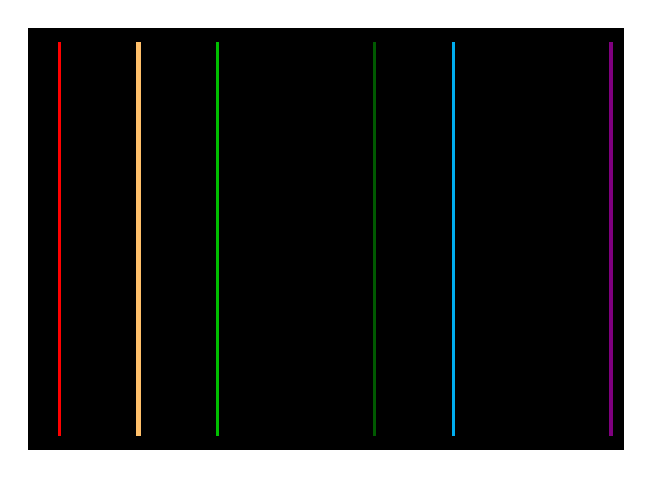
\begin{tikzpicture}[background rectangle/.style={fill=black}, show background rectangle]
			\def\len{5}
			\def\rot{10}
			\def\orange{11}
			\def\gruen{12}
			\def\dgruen{14}
			\def\tuerkis{15}
			\def\lila{17}
			\draw[-,very thick, color=red] (\rot,0) -- (\rot,\len) node [pos=.5,sloped,above] {};
			\draw[-,ultra thick, color={rgb:orange,2;yellow,2;pink,5}] (\orange,0) -- (\orange,\len) node [pos=.5,sloped,above] {};
			\draw[-,very thick, color=black!25!green] (\gruen,0) -- (\gruen,\len) node [pos=.5,sloped,above] {};
			\draw[-,very thick, color=black!65!green] (\dgruen,0) -- (\dgruen,\len) node [pos=.5,sloped,above] {};
			\draw[-,very thick, color=cyan] (\tuerkis,0) -- (\tuerkis,\len) node [pos=.5,sloped,above] {};
			\draw[-,very thick, color=violet] (\lila,0) -- (\lila,\len) node [pos=.5,sloped,above] {};
		\end{tikzpicture}
		\caption{Skizze der erkenntlichen Spektralinien der Natriumdampflampe nach einem Prisma.}
		\label{fig_draw}
	\end{figure}
	\subsubsection*{Gitter}
	Die Winkel Spektrallinien lassen sich mit der Formel aus der Einführung in Wellenlängen umrechnen:
	\begin{equation}
		\lambda = \frac{g \cdot \sin{\vartheta_m}}{m}
		\label{eq_lambda}
	\end{equation}
	\begin{equation}
		u(\lambda) = \left|\frac{g \cdot \cos{\vartheta_m} \cdot u(\vartheta_m)}{m}\right|
	\end{equation}
 	Dabei ist $g$ die Gitterkonstante und $\vartheta_m$ der Beugungswinkel des $m$-ten Beugungsmaximums.
	In \cref{fig_natrium} sind für die Gitter $g=1/\SI{300}{mm}$ und $g=1/\SI{600}{mm}$ die aus den Winkeln resultierenden Wellenlängen verschiedener Ordnungen dargestellt.
	
	\begin{figure}[H] 
		\includegraphics[width=1\textwidth]{fig_natrium} 
		\centering
		\caption{Die aus dem Beugungswinkel der Maxima resultierenden Wellenlängen einer Natriumdampflampe sind abgebildet.
		Die Unsicherheit bei der roten Messpunkte ist kleiner als die Symbolgröße.}
		\label{fig_natrium}
		\centering
	\end{figure}
	\subsubsection{Heliumlampe} \label{ss_helium}
	In der Einführung ist eine Tabelle zum Kalibrieren des Spektrometers gegeben. %TODO Soll man die angeben, nach Mühlenstrodt scheinbar ja
	Die Wellenlängen mit einer Intensität größer gleich 100 wurden als die sichtbaren eingestuft, da dies sechs Spektrallinien ergibt und sechs Spektrallinien beobachtet wurden.
	Die Kalibrationstabelle beinhaltet zwei rote Spektrallinien, jedoch wurde im Experiment nur eine gemessen.
	Außerdem ließ sich die am wenigsten intensive Spektrallinie farblich keiner passenden Wellenlänge eindeutig zuordner, deshalb ergibt sich \cref{fig_helium} aus fünf Messpunkten.
	Nach \cref{eq_lambda} würde man eine Sinus-Abhängigkeit erwarten. 
	Eine linearer Fit liegt jedoch deutlich genauer an den Messpunkten, weshalb dieser dienlicher als Kalibrationskurve ist.
	Es ist auffählig, dass der Vorfaktor $a$ des Sinus-Fits den erwarteten Wert von 1/\SI{600}{mm} beinhaltet. 
	Aus dem $a$ würde eine Gitterkonstante innerhalb des Bereichs von 1/\SI{577}{mm} bis 1/\SI{613}{mm} folgen.
	

	\begin{figure}[H] 
		\includegraphics[width=1\textwidth]{fig_helium} 
		\centering
		\caption{Die Wellenlängen der Kalibrationstabelle sind gegen die gemessenen Winkel der zugehörigen Spektrallinien aufgetragen.
		Die blaue Funktion ist ein Linearer Fit.
		Die rote Funktion ist ein Sinus-Fit.}
		\label{fig_helium}
		\centering
	\end{figure}
	\subsubsection{Energiesparlampe}
	Mithilfe der in \cref{ss_helium} bestimmten Kalibrationskurve lassen sich die Wellenlängen der Spektrallinien der Energiesparlampe ermitteln.
	Diese sind in \cref{fig_spar} dargestellt.


	\begin{figure}[H] 
		\includegraphics[width=1\textwidth]{fig_spar} 
		\centering
		\caption{Spektrallinien der Energiesparlampe. 
		Es wurden lediglich Maxima der ersten Beugungsordnung beobachtet.}
		\label{fig_spar}
		\centering
	\end{figure}	

	\subsubsection{Leuchtdioden}
	In \cref{fig_led} wurde ein linearer Fit berechnet. 
	Dessen Steigung sollte $hc$ betragen.
	Durch Division von $A$ durch $c$ lässt sich das Planksche Wirkungsquantum mit \SI{5,39 +- 0,92 e-15}{eVs} bestimmen.


	\begin{figure}[H] 
		\includegraphics[width=1\textwidth]{fig_led} 
		\centering
		\caption{Die Spannung, ab der die Diode zu leichten beginnt, ist gegen den Kehrwert des Maximums der Emissionswellenlänge aufgetragen.}
		\label{fig_led}
		\centering
	\end{figure}	
	%TODO Berechung nach Aufgabenstellung
	
	\subsection{Diskussion}
	%TODO Bezug/Nutzen oder sonst was
	%TODO auch hier die Hypothese wiederholen
	%TODO keine Messwerte hier, nach manchen Menschen, zumindest "direkt" erstellte Diagramme net hier, auch wenn Lesbarkeit-bla
	
	\section{Schlussfolgerung}
	%TODO Rückgriff auf Hypothese und drittes Nennen dieser
	
	%TODO Quellen zitieren, Websiten mit Zugriffsdatum
	%TODO Verweise auf das Laborbuch (sind erlaubt)
	%TODO Tabelle + Bilder mit Beschriftung
	%\printbibliography
\end{document}
